%% March 2018
%%%%%%%%%%%%%%%%%%%%%%%%%%%%%%%%%%%%%%%%%%%%%%%%%%%%%%%%%%%%%%%%%%%%%%%%%%%%
% AGUJournalTemplate.tex: this template file is for articles formatted with LaTeX
%
% This file includes commands and instructions
% given in the order necessary to produce a final output that will
% satisfy AGU requirements, including customized APA reference formatting.
%
% You may copy this file and give it your
% article name, and enter your text.
%
%
% Step 1: Set the \documentclass
%
% There are two options for article format:
%
% PLEASE USE THE DRAFT OPTION TO SUBMIT YOUR PAPERS.
% The draft option produces double spaced output.
%

%% To submit your paper:
\documentclass[draft,linenumbers]{agujournal2018}
\usepackage{apacite}
\usepackage{url} %this package should fix any errors with URLs in refs.
%%%%%%%
% As of 2018 we recommend use of the TrackChanges package to mark revisions.
% The trackchanges package adds five new LaTeX commands:
%
%  \note[editor]{The note}
%  \annote[editor]{Text to annotate}{The note}
%  \add[editor]{Text to add}
%  \remove[editor]{Text to remove}
%  \change[editor]{Text to remove}{Text to add}
%
% complete documentation is here: http://trackchanges.sourceforge.net/
%%%%%%%


%% Enter journal name below.
%% Choose from this list of Journals:
%
% JGR: Atmospheres
% JGR: Biogeosciences
% JGR: Earth Surface
% JGR: Oceans
% JGR: Planets
% JGR: Solid Earth
% JGR: Space Physics
% Global Biogeochemical Cycles
% Geophysical Research Letters
% Paleoceanography and Paleoclimatology
% Radio Science
% Reviews of Geophysics
% Tectonics
% Space Weather
% Water Resources Research
% Geochemistry, Geophysics, Geosystems
% Journal of Advances in Modeling Earth Systems (JAMES)
% Earth's Future
% Earth and Space Science
% Geohealth
%
% ie, \journalname{Water Resources Research}

\journalname{Geohealth}


% tightlist command for lists without linebreak
\providecommand{\tightlist}{%
  \setlength{\itemsep}{0pt}\setlength{\parskip}{0pt}}



\usepackage{soulutf8}
\usepackage{float}
\floatplacement{figure}{H}
\usepackage{amsmath}
\usepackage{booktabs}
\usepackage{caption}
\usepackage{longtable}

\begin{document}


%% ------------------------------------------------------------------------ %%
%  Title
%
% (A title should be specific, informative, and brief. Use
% abbreviations only if they are defined in the abstract. Titles that
% start with general keywords then specific terms are optimized in
% searches)
%
%% ------------------------------------------------------------------------ %%

% Example: \title{This is a test title}

\title{Geographic Characterization of Benzene Plumes in California}

%% ------------------------------------------------------------------------ %%
%
%  AUTHORS AND AFFILIATIONS
%
%% ------------------------------------------------------------------------ %%

% Authors are individuals who have significantly contributed to the
% research and preparation of the article. Group authors are allowed, if
% each author in the group is separately identified in an appendix.)

% List authors by first name or initial followed by last name and
% separated by commas. Use \affil{} to number affiliations, and
% \thanks{} for author notes.
% Additional author notes should be indicated with \thanks{} (for
% example, for current addresses).

% Example: \authors{A. B. Author\affil{1}\thanks{Current address, Antartica}, B. C. Author\affil{2,3}, and D. E.
% Author\affil{3,4}\thanks{Also funded by Monsanto.}}

\authors{
Andrew R. Murray
\affil{1, 2}
\thanks{Andrew's thanks}
Diego Riveros-Iregui
\affil{1}
\thanks{Current address: Some other place, Germany}
Alexander Hall
\affil{3}
Fran Kremer
\affil{3}
}


% \affiliation{1}{First Affiliation}
% \affiliation{2}{Second Affiliation}
% \affiliation{3}{Third Affiliation}
% \affiliation{4}{Fourth Affiliation}

\affiliation{1}{The University of North Carolina - Chapel Hill}
\affiliation{2}{Oak Ridge Associated Universities}
\affiliation{3}{U.S. Environmental Protection Agency Office of Research
and Development}
%(repeat as many times as is necessary)

%% Corresponding Author:
% Corresponding author mailing address and e-mail address:

% (include name and email addresses of the corresponding author.  More
% than one corresponding author is allowed in this LaTeX file and for
% publication; but only one corresponding author is allowed in our
% editorial system.)

% Example: \correspondingauthor{First and Last Name}{email@address.edu}
\correspondingauthor{Andrew Murray}{Murray.AndrewR@epa.gov}

%% Keypoints, final entry on title page.

%  List up to three key points (at least one is required)
%  Key Points summarize the main points and conclusions of the article
%  Each must be 100 characters or less with no special characters or punctuation

% Example:
% \begin{keypoints}
% \item	List up to three key points (at least one is required)
% \item	Key Points summarize the main points and conclusions of the article
% \item	Each must be 100 characters or less with no special characters or punctuation
% \end{keypoints}

\begin{keypoints}
\item Spatio-temporal patterns of benzene plumes are still poorly
understood.
\item Most plumes are not spatially captured by groundwater testing.
\item Better models are needed to inform monitoring well selection for
leaking sites.
\end{keypoints}

%% ------------------------------------------------------------------------ %%
%
%  ABSTRACT
%
% A good abstract will begin with a short description of the problem
% being addressed, briefly describe the new data or analyses, then
% briefly states the main conclusion(s) and how they are supported and
% uncertainties.
%% ------------------------------------------------------------------------ %%

%% \begin{abstract} starts the second page

\begin{abstract}
Underground storage tanks are tanks buried underground for the purpose
of storing and dispensing a wide range of hazardous products. The
primary use for these tanks are the storing and dispensing of fuel
products such as gasoline and diesel. In the United States there are
currently 540,000 open (in operation) tanks. Since 2000, there have been
more than 118,000 reported releases. When fuel products release into the
ground or onto the surface they can contaminate local soil and
groundwater resources, as well as pollute the air by means of vapor
intrusion. Petroleum hydrocarbons, which are known carcinogens, pose a
threat to human and environmental health. They can persist in the
environment for decades, and can contaminate drinking water to unsafe
levels before becoming detectable by smell or taste. Benzene is the most
common petroleum hydrocarbon found in fuel products and several studies
have been conducted on it's potential for movement in the environment,
however these studies all generally contain a limited number of sites
within a limited geographic area and much remains to be understood
related to environmental drivers.
\end{abstract}
\section{Introduction}

Benzene, a carcinogenic component of petroleum products such as gasoline
is known to be released into the environment as the result of leaking
underground storage tanks (LUST). There are currently about 540,000
active petroleum UST systems and a backlog of 62,000 LUST sites in the
United States \citep{ustperformance} . The definition of a leaking
underground storage tank can vary depending on which state or federal
regulations you consider. The federal government considers reportable
quantities of petroleum products to be anything over 25 gallons, or a
spill that cannot be cleaned up within 24 hours \citep{coderegs}. Many
studies have been done on benzene plume length and attenuation
\citep[e.g.,][]{connor2015, kamath2012, shih2004evaluation}. However
much is still unknown about the behavior and extent of benzene plumes.
For example, while most papers focus on distance (one-dimensional),
fewer characterize total impacted area (two-dimensional), and those that
do, typically focus on only a relative few contaminated sites. A review
paper on studies on benzene plume length showed that research on this
area included between 22 to 289 LUST sites per study \citep{connor2015}.
\citet{mchugh2014progress} included over 4,000 LUST sites, however this
was not focused on distance or area but rather trends in concentration
over time. A key reason for the limited number of sites included in
these studies is data availability. Although states are required to test
and characterize sites contaminated or suspected to be contaminated by
leaking underground storage tanks, very limited amounts of these data
are made public. In most of the papers cited here, authors accumulated
limited amounts of field data from multiple agencies and sources. An
exception to this is California's geotracker database, the largest
publicly available database of its kind, which includes field data for
leaking underground storage tank cleanup sites dating back to 2000.

There has yet to be a study done on benzene plume areas that
sufficiently considers a large number of field studies, geographic
diversity of sites, and two-dimensional plume shape. Further, no study
has been able to offer insight into estimating plume locations, which
could help to make future testing campaigns more efficient and accurate.
In this paper, we aim to consider the largest number of field studies to
date and to characterize benzene plume shapes and distances. To do this,
we use data obtained from California's GeoTracker database and compare
geotracker data with the findings of \citet{connor2015} to determine how
a larger and more diverse sample size supports or disagrees with the
findings of other studies. We then characterize two-dimensional benzene
plume areas to determine the shape and distribution of benzene plumes.
Finally, we determine how effective monitoring wells are at completely
capturing benzene plumes in California. These essential investigations
will help to determine if we can more accurately estimate plume extents
in the future and suggest possible ways to make LUST site investigations
and monitoring campaigns more efficient. California's geotracker
database is a valuable and generally untapped resource of information
which should be a model for other state agencies which are responsible
for the cleanup of LUST sites.

\section{Materials and Methods}

\subsection{California release definitions}

The definition of a release varies from state to state, however all
states must report releases that meet or exceed the criteria of the
federal reporting requirements. Many releases do not meet this threshold
but may still appear in California's geotracker database. California
defines a release as:

\begin{quote}
``{[}A{]} spill or overfill of a hazardous substance that meets both of
the following conditions: (1) The spill or overfill occurs while the
hazardous substance is being placed in an underground storage tank. (2)
The spill or overfill is due to the use of improper equipment, faulty
equipment, operator error, or inattention or overfilling
\citep{careport25295.5}''
\end{quote}

In California, operators are not required to report a release or spill
if they are ``able to clean up within eight hours after the release was
detected or should reasonably have been detected, and which does not
escape from the secondary containment, does not increase the hazard of
fire or explosion, and does not cause any deterioration of the secondary
containment of the underground storage tank.'' However the operator must
record the incident in monitoring reports \citep{careport25294}. If
these thresholds are exceeded, the operator must report the spill to the
apropriate state agency \citep{careport25295}.

\subsection{Geotracker}

The data obtained from GeoTracker contains groundwater measurements from
5293 unique leaking underground storage sites. Previous Studies have
proposed that the maximum travel distance of benzene in the ground is
between 300 and 1,700 feet and that the 90th percentile of benzene plume
lengths is between 345 and 425 feet \citep{connor2015}. There are more
than 500,000 underground storage tanks in the United States. For about
every 7 active tanks, one will report a release in it's lifetime
\citep{ustperformance}. Several studies exist which examine the
distances and depths of benzene migration in the vadose zone, however
most studies lack robust numbers of study sites as cleanup data is not
widely available. Further, no studies exist which examine the
two-dimensional footprints of benzene plumes at large scales or
monitoring well placement relative to leak points. We examine over
three-thousand leaking underground storage tank (LUST) site cleanups in
California which exhibited measurable benzene plumes and determine
characteristics of their spatial extents, flow directions and whether
the monitoring wells used at the sites adequately capture plume extents.
We determine (a) if geotracker data supports previous studies in
1-dimensional maximum plume distance. (b) from a spatial perspective, if
site monitoring efforts are effectively capturing 2-dimensional benzene
plumes, (c) if benzene plumes have a pronounced shape to them and the
size of impacted areas, and (d) discuss what can be done to make plume
monitoring more effective and efficient in the future.

\subsection{Determining Plume Length}

There is no set definition for the point of origin for an underground
storage tank release. This is common as most releases are discovered as
a result of tank removal and it is often unclear from exactly where a
release occurred. While the geotracker database does provide xy
locations for both `UST / UST pit' and `former UST' locations, these
data only exist at less than 200 of LUST cleanup sites. Therefore, we
define the point of release as the point where benzene concentration was
the highest at a given site. If there were multiple measurements of the
maximum concentration at different points, the earliest measurement was
used. As in \citet{connor2015}, the plume is defined as the total area
above two separate thresholds, 5 ug/L and 10 ug/L to match with
definitions used by previous studies. To be clear, the current federal
MCL for benzene is 5 ug/L.

\subsection{Evaluating Capture of Plumes by Monitoring Wells}

We look at plume extents compared to monitoring extents to determine if
plumes are completely captured by monitoring wells or if concentrations
greater than 5 ug/L are possibly extending beyond monitoring wells. To
test this, we create convex hulls \citep{sf} of the monitoring wells
which measured \(\ge 5 ug/L\) for every testing event for every site and
also convex hulls for monitoring wells for every site. We define samples
taken in a specific testing event as a time when the origination point
was tested, and every sample taken from every well within ± 28 days.

\begin{figure}[h]
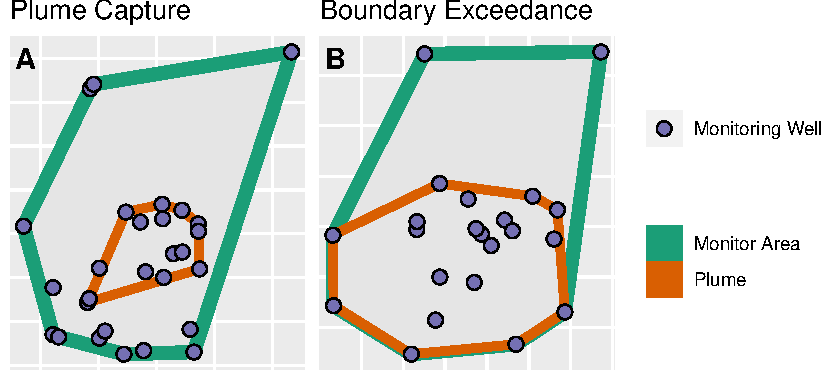
\includegraphics{CA_Benzene_Plumes_files/figure-latex/exceedsExample-1} \caption{Example of Plumes that are completely captured by monitoring wells (A) and plumes which likely travel beyond he extent of moniotring wells (B).}\label{fig:exceedsExample}
\end{figure}

\subsection{Normalizing Plume Direction}

We map out the distribution of monitoring wells relative to the mean
linear direction of a benzene plume. To determine the mean linear
direction of benzene movement through the ground, we use weighted vector
addition to determine the mean angle of flow in degrees from north. We
then artificially rotate the plumes so that they are normalized to one
direction (due north) and overlay them to map out monitoring wells
relative to the leak point and direction of flow and regardless to
actual location. All analysis was done in using the R statistical
language \citep{R} within RStudio \citep{RStudio}. Coordinate math was
done using sf \citep{sf} and bearing directions were calculated using
stplanr \citep{stplanr}. Data cleaning relied on the tidyverse package
\citep{tidyverse}. To weight monitoring wells, benzene concentrations
were multiplied by the distance in meters of the monitoring well from
the LOP. Lines were then created using existing bearings for each
monitoring well from the LOP and lengths from weighted distances. Lines
were then drawn end to end and the mean linear direction was calculated
as the bearing between the LOP and the end vertex of the final weighted
line.

\begin{figure}[h]
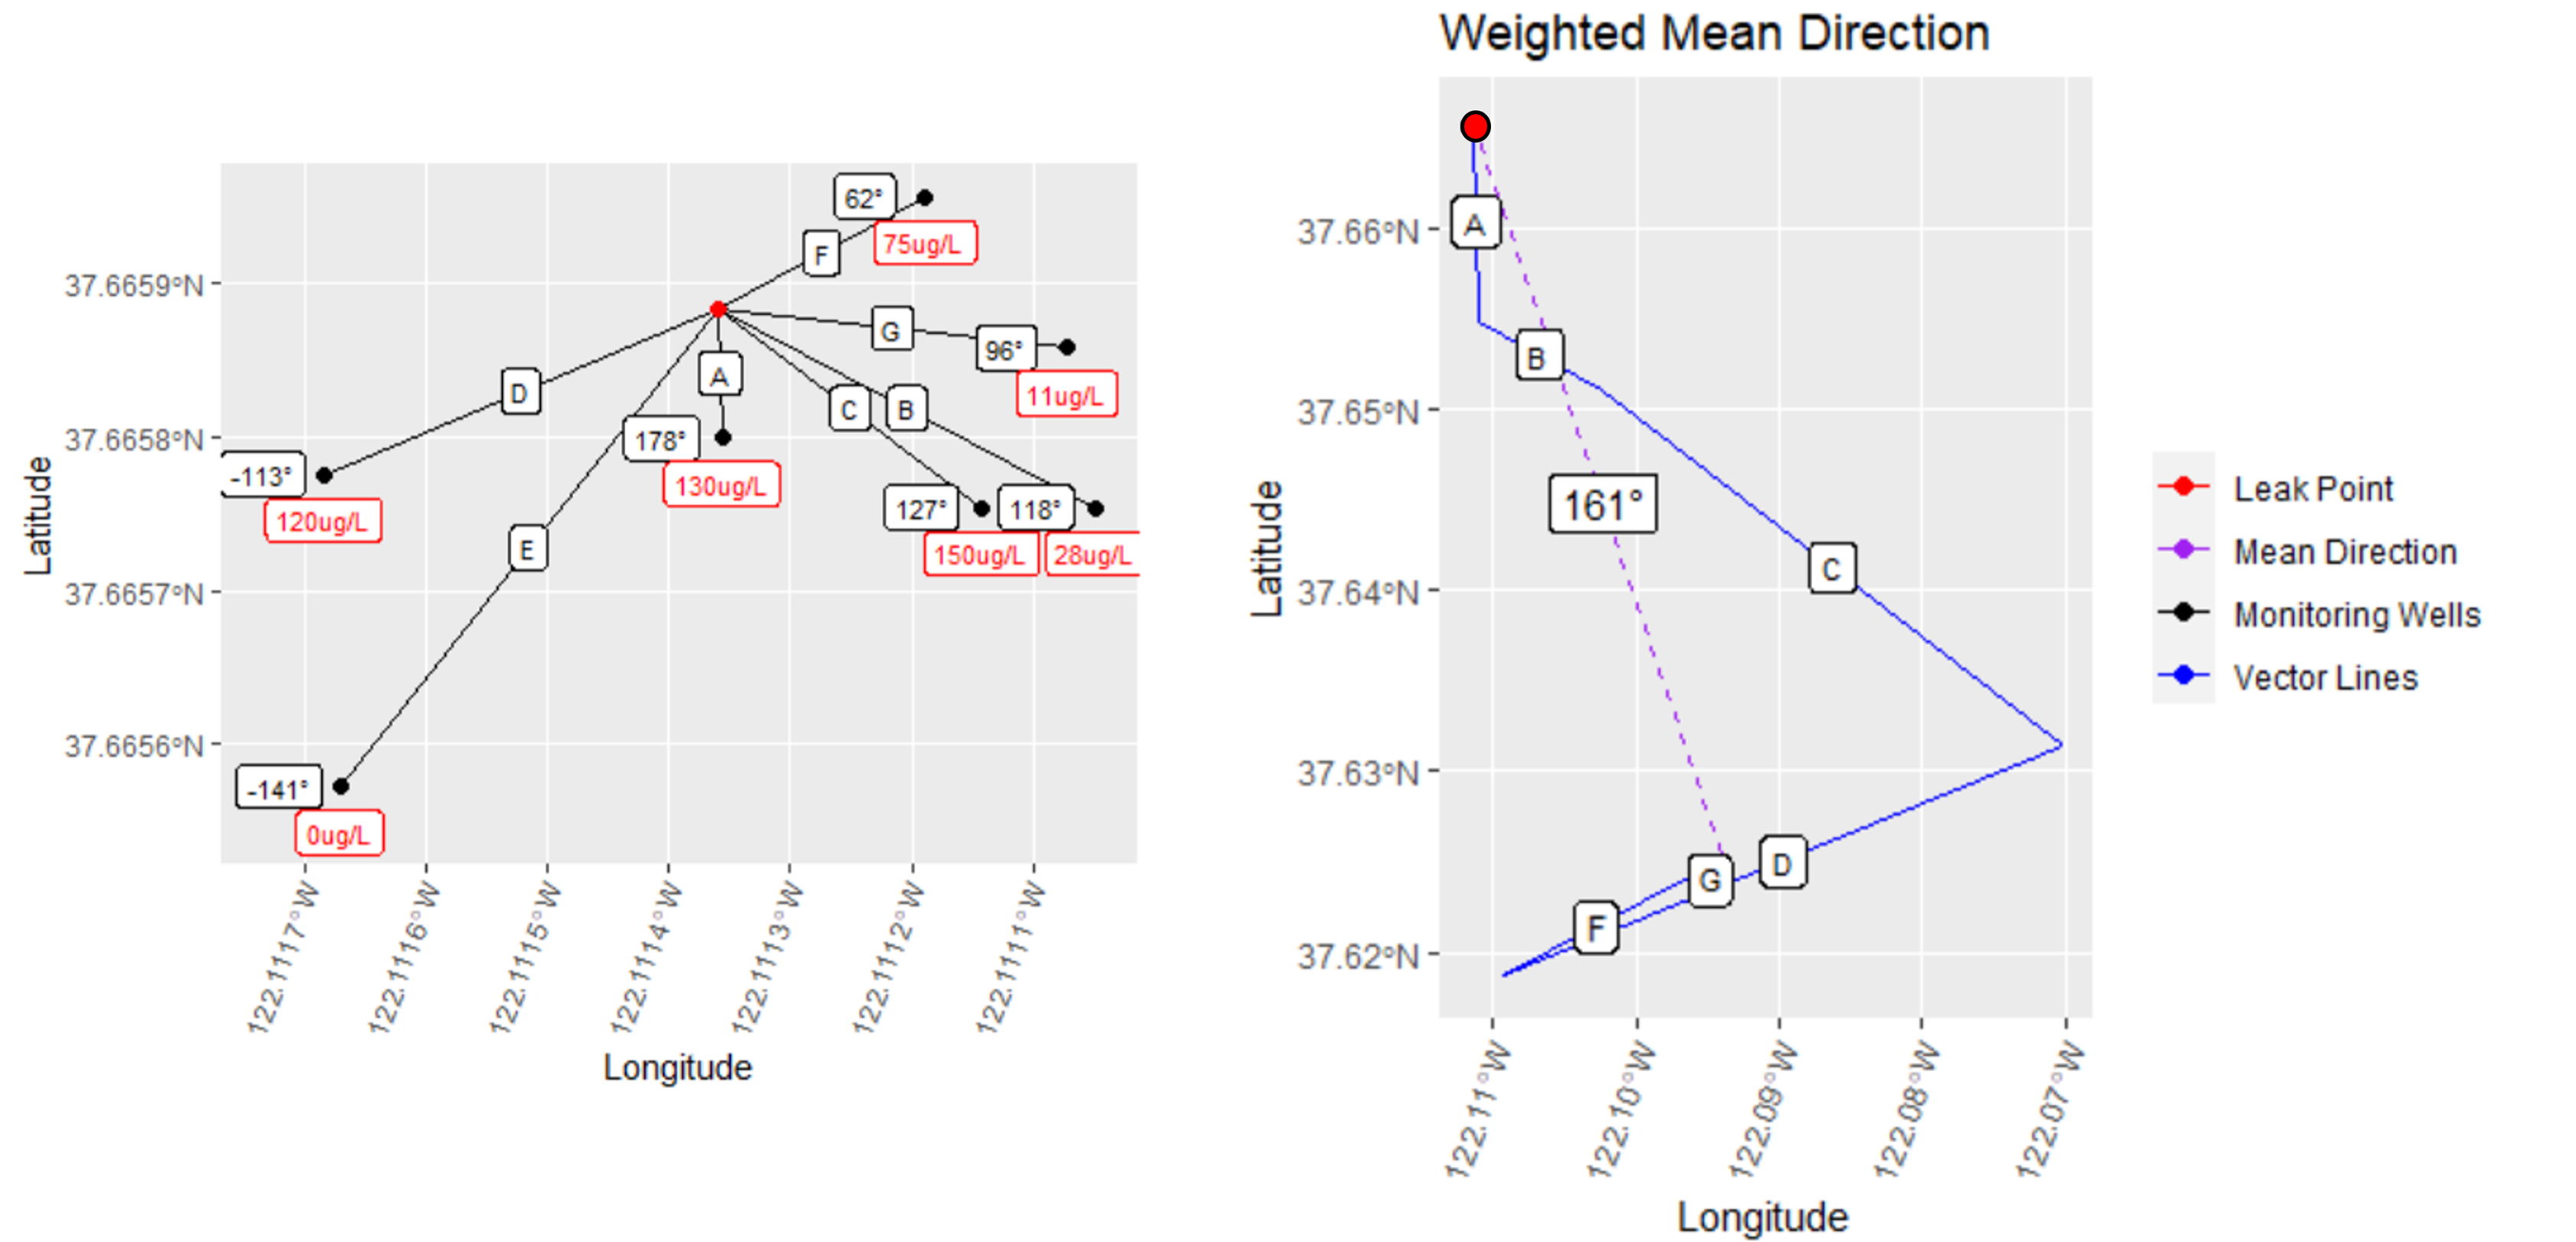
\includegraphics[width=400px,]{img/meanDirection} \caption{Illustration of mean direction calculation. Panel A shows actual locations and concentrations of benzene relative to LOP. Panel B shows weighted vector math result with mean linear direction calculation.}\label{fig:fig1}
\end{figure}

We included all benzene samples in geotracker which were taken at LUST
cleanup sites and were analyzed as either ug/L or mg/L (91.3\% of all
samples). In total, we included 1.8 million benzene samples from 104,254
geographically unique sampling points at 8,409 LUST cleanup sites. 7,058
LUST cleanup sites had benzene concentrations greater than the MCL (5
ug/L).

\section{Results}

\subsection{Maximum Plume Distance}

Figure 2 shows the maximum distance benzene was measured from the point
of origination.

\begin{figure}[h]
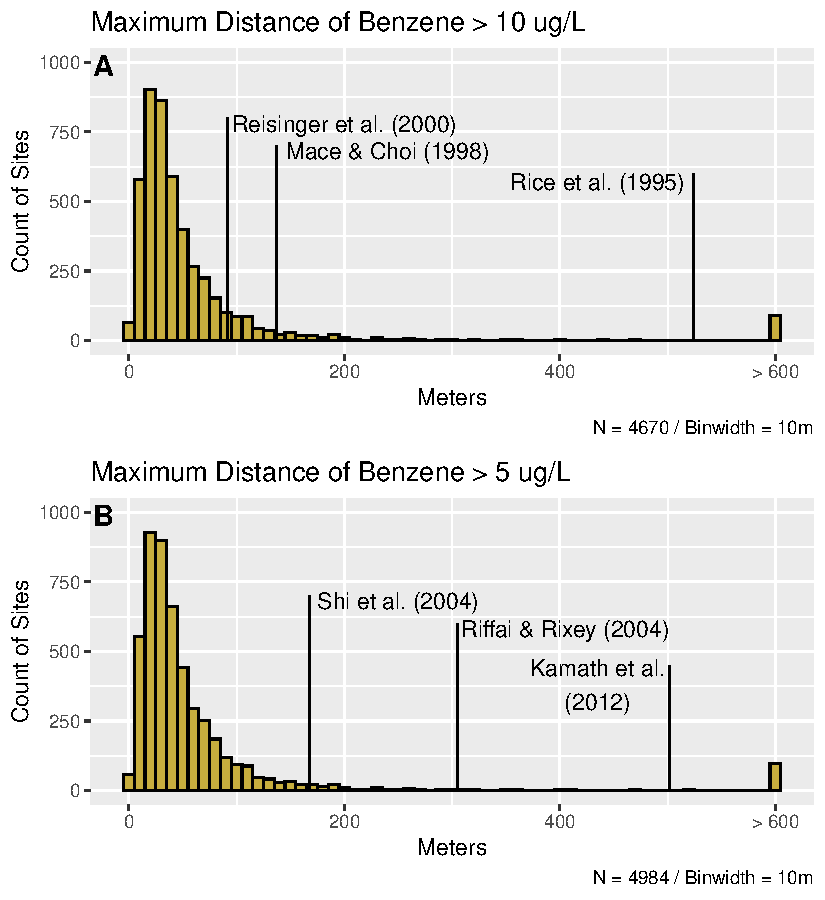
\includegraphics{CA_Benzene_Plumes_files/figure-latex/maxDist-1} \caption{Maximum calculated distance of benzene plumes in meters using a threshold of 10 ug/L.}\label{fig:maxDist}
\end{figure}

\begin{figure}[h]
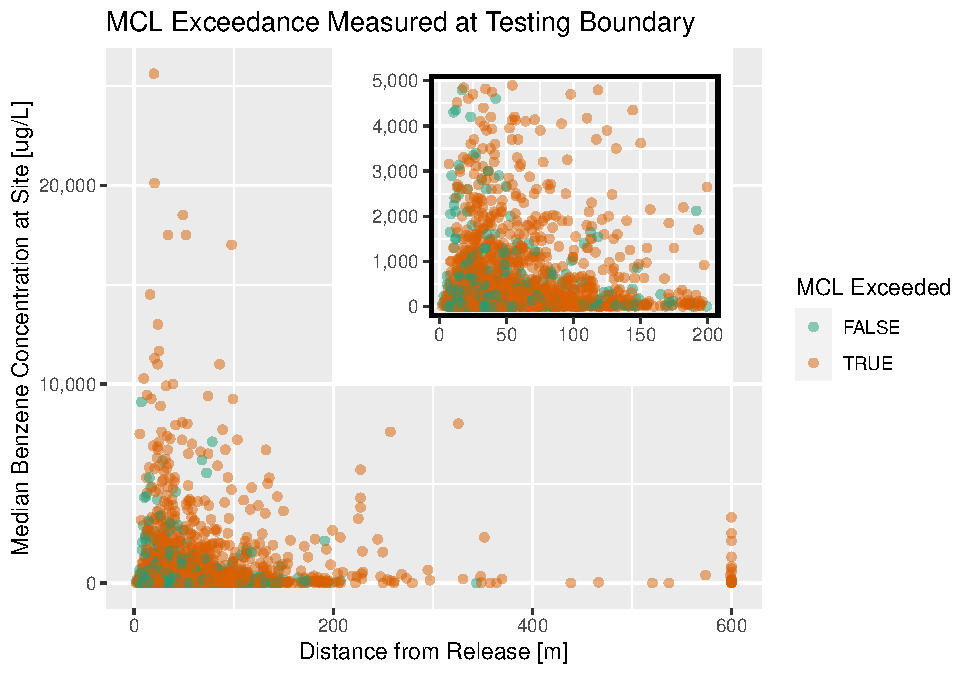
\includegraphics{CA_Benzene_Plumes_files/figure-latex/boundaryExceedance-1} \caption{Exceedance classification for every LUST cleanup site in California with more than 3 sampling points > 5 ug/L shown with maximum plume distance and median concentration at site.}\label{fig:boundaryExceedance}
\end{figure}

2,597 of 3,300 cleanup sites had an exceedance of 5 ug/L at the testing
boundary (78.7\%)

\subsection{Overlayed Plumes and Study Areas}

\begin{itemize}
\tightlist
\item
  We found 4,202 plumes with at least 3 points with benzene
  concentrations \textgreater= 5 ug/L. We calculated mean linear
  direction of benzene flow and rotated each plume to due north. Each
  plume was overlaid by shifting the leak origination point to the
  coordinates (0,0) in the California albers projection.
\end{itemize}

All Plumes and Study Areas

\begin{figure}[h]
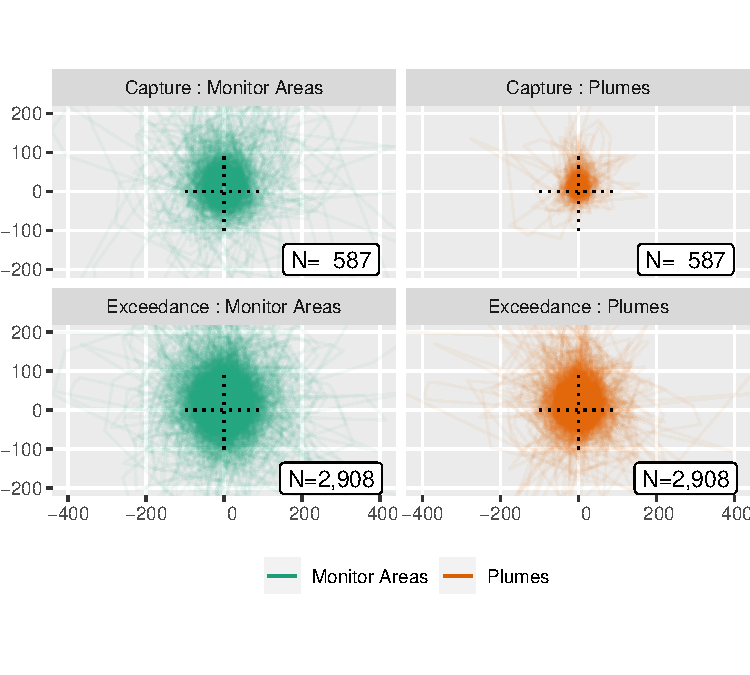
\includegraphics{CA_Benzene_Plumes_files/figure-latex/AllplumeAreas-1} \caption{Please caption every figure}\label{fig:AllplumeAreas}
\end{figure}

\subsection{Plumes entirely within testing boundary}

\begin{figure}[h]
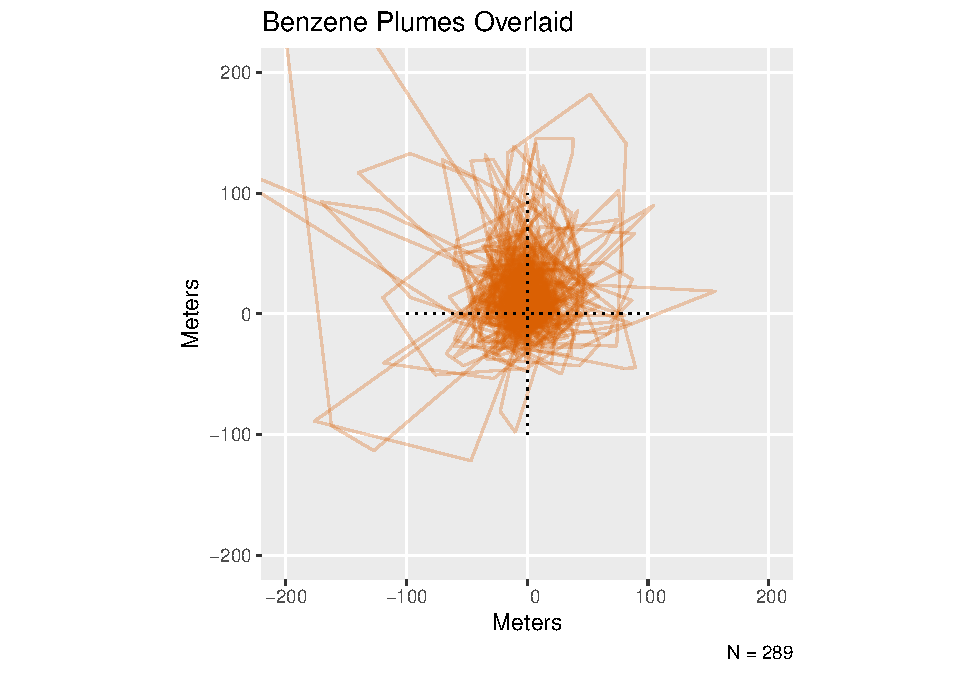
\includegraphics{CA_Benzene_Plumes_files/figure-latex/plumesinBoundary-1} \caption{Please caption every figure}\label{fig:plumesinBoundary}
\end{figure}

\subsection{Are plumes that are completely captured, significantly
smaller than plumes that have boundary exceedance?}

\begin{figure}[h]
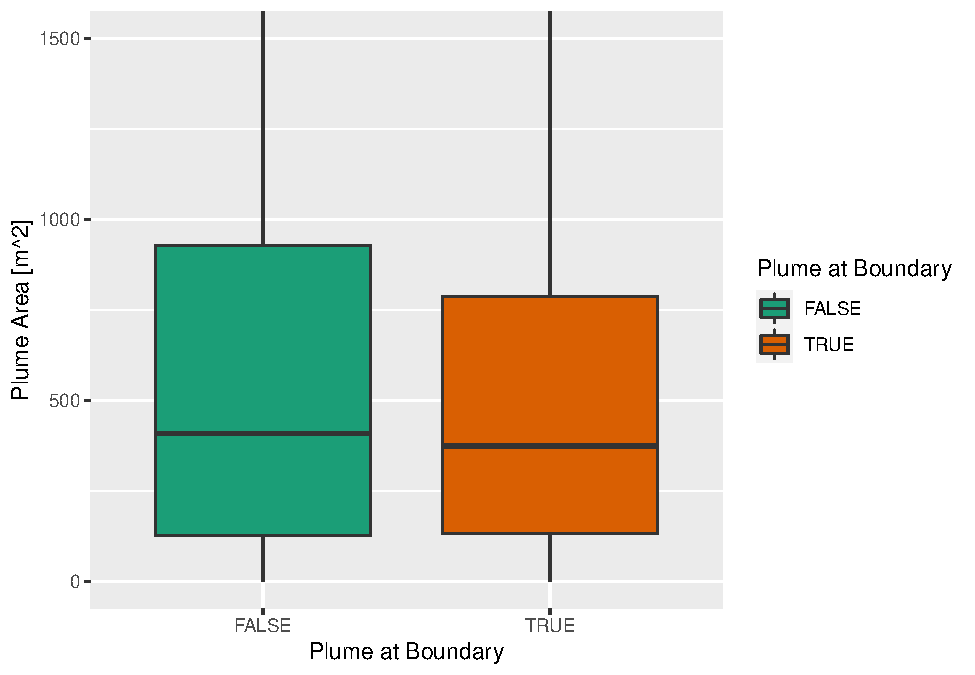
\includegraphics{CA_Benzene_Plumes_files/figure-latex/plumeAreaCompare-1} \caption{Please caption every figure}\label{fig:plumeAreaCompare}
\end{figure}

This plot tells us that when plumes are completely captured (spatially)
that they are not larger than if plumes extend to the boundary of a
monitoring network. This suggests that plumes, in general, are larger
than the data suggests. Measured plumes get larger as monitored areas
get larger.

\subsection{Wilcox Test}

Wilcox Results:

\captionsetup[table]{labelformat=empty,skip=1pt}
\begin{longtable}{lllrrrr}
\toprule
.y. & group1 & group2 & n1 & n2 & statistic & p \\ 
\midrule
Plume\_Area & FALSE & TRUE & 703 & 2597 & 646968 & 1.82e-32 \\ 
\bottomrule
\end{longtable}

Effect Size:

\captionsetup[table]{labelformat=empty,skip=1pt}
\begin{longtable}{rc}
\toprule
effsize & magnitude \\ 
\midrule
0.206528 & small \\ 
\bottomrule
\end{longtable}

\section{Conclusions}

\begin{itemize}
\item
  Plumes are not being effectively captured by monitoring wells

  \begin{itemize}
  \item
    When plumes are completely captured by monitoring wells, the plumes
    tend to be smaller, suggesting that larger plumes are not being
    reflected in the data and that, in general, monitoring wells are
    placed at fixed distances.
  \item
    As Plumes get larger, they are less likely to be captured by
    monitoring wells
  \end{itemize}
\item
  There is no clear issue with the radial coverage from a leaking point

  \begin{itemize}
  \tightlist
  \item
    The data does not support the hypothesis that monitoring wells are
    not placed in directions other than the dominant flow direction of
    benzene.
  \end{itemize}
\item
  Benzene plumes appear to exhibit radial characteristics with a skewed
  dominant flow direction.
\end{itemize}

\section{NOTES}

\begin{verbatim}
## New names:
## * `` -> ...1
\end{verbatim}

\begin{verbatim}
## Rows: 1000 Columns: 3
## -- Column specification --------------------------------------------------------
## Delimiter: ","
## dbl (3): ...1, Distance_m, countWells
## 
## i Use `spec()` to retrieve the full column specification for this data.
## i Specify the column types or set `show_col_types = FALSE` to quiet this message.
\end{verbatim}

\begin{figure}[h]
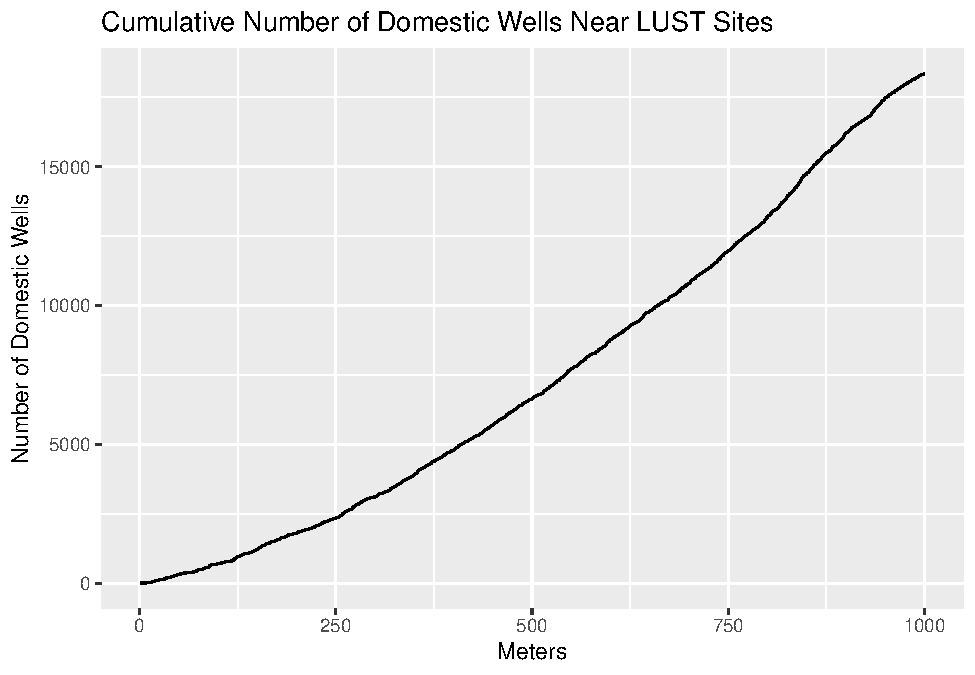
\includegraphics{CA_Benzene_Plumes_files/figure-latex/unnamed-chunk-2-1} \caption{Please caption every figure}\label{fig:unnamed-chunk-2}
\end{figure}

\begin{verbatim}
## Warning: Removed 178 rows containing missing values (geom_point).
\end{verbatim}

\begin{figure}[h]
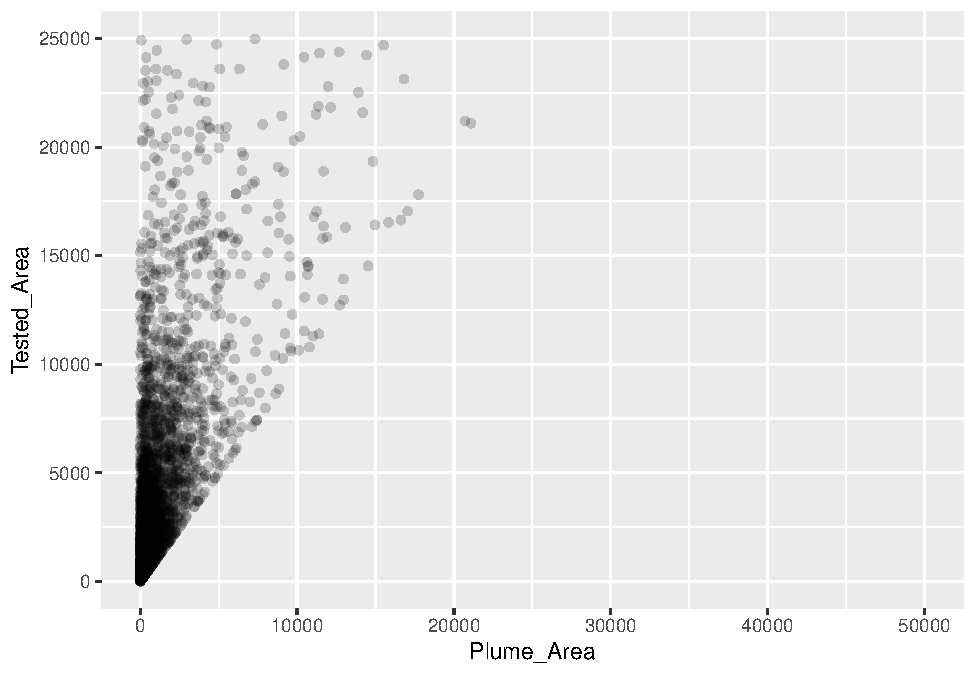
\includegraphics{CA_Benzene_Plumes_files/figure-latex/unnamed-chunk-3-1} \caption{Please caption every figure}\label{fig:unnamed-chunk-3}
\end{figure}

Driving Questions:

\begin{itemize}
\item
  Does our data support the conclusions form other studies on plume
  length?
\item
  From a spatial perspective, are site monitoring efforts effectively
  capturing the complete extent of benzene plumes?
\item
  What are the shapes of plumes? Are they flowing in a single direction,
  or are they spreading outwards in many directions?
\item
  Are there systematic issues in the way that monitoring wells are
  located? Are we looking in the right places?
\item
  Can we contribute to better monitoring in the future?
\end{itemize}

\subsection{Plot Points where MCL is exceeded at boundary}

In the plot below, we show every point where the mcl was exceeded at a
testing boundary. If there were a systematic pattern of areas where
monitoring wells were not being drilled, we would expect to see a more
concentrated number of points. For example, if technicians were not
looking far enough away from leak points in the opposite direction of
the mean linear flow direction of benzene, we would expect to see a
concentration of points in the area of y \textless{} 0. However, we do
not see any such pattern. Instead, we see a pattern similar to the
general plume shape. This indicates that there is no systematic issue
with where monitoring wells are placed, at least there is no area that
is being missed more than any other.

\begin{figure}[h]
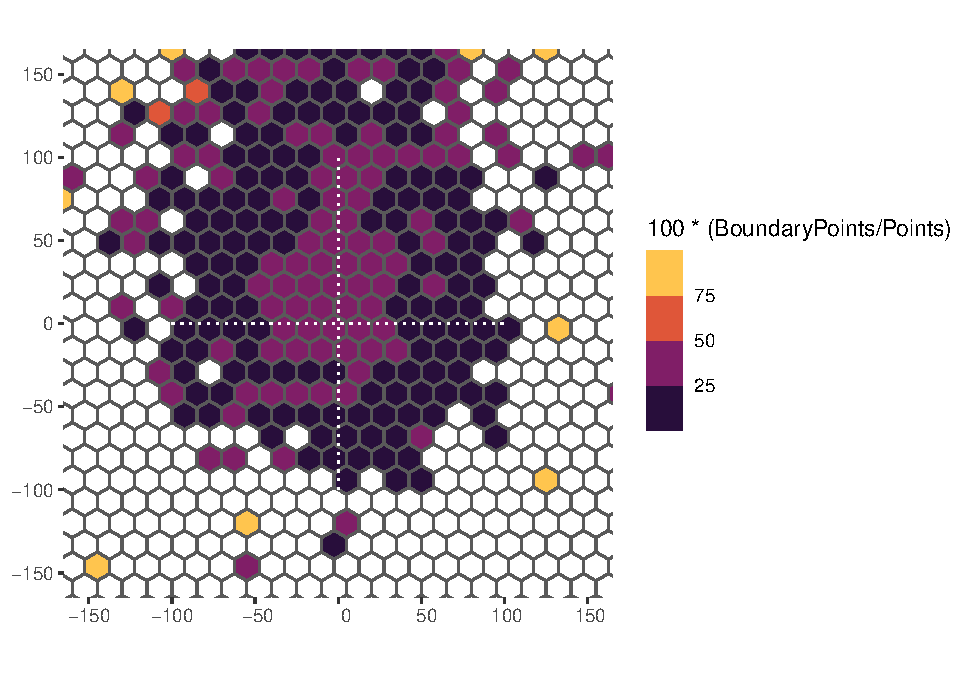
\includegraphics{CA_Benzene_Plumes_files/figure-latex/boundaryPts-1} \caption{Please caption every figure}\label{fig:boundaryPts}
\end{figure}

\appendix
\section{Here is a sample appendix}

Optional Appendix goes here

Optional Glossary, Notation or Acronym section goes here:

Glossary is only allowed in Reviews of Geophysics

\begin{glossary}
\term{Term}
 Term Definition here
\term{Term}
 Term Definition here
\term{Term}
 Term Definition here
\end{glossary}

\begin{acronyms}
\acro{UST}
 Underground Storage Tanks
\acro{LUST}
 Leaking Underground Storage Tank
\end{acronyms}

\begin{notation}
\notation{$a+b$} Notation Definition here
\notation{$e=mc^2$}
Equation in German-born physicist Albert Einstein's theory of special
relativity that showed that the increased relativistic mass ($m$) of a
body comes from the energy of motion of the body—that is, its kinetic
energy ($E$)—divided by the speed of light squared ($c^2$).
\end{notation}

\acknowledgments

The acknowledgments must list: A statement that indicates to the reader
where the data supporting the conclusions can be obtained (for example,
in the references, tables, supporting information, and other databases).

All funding sources related to this work from all authors

Any real or perceived financial conflicts of interests for any author

Other affiliations for any author that may be perceived as having a
conflict of interest with respect to the results of this paper.

It is also the appropriate place to thank colleagues and other
contributors.

AGU does not normally allow dedications.

\bibliography{references.bib}


\end{document}
